% !TEX root = ./main.tex

\section{Determining and removing an equilibration or `burn-in' portion of a trajectory}
\label{sec:equil}

\begin{figure}
  \centering
  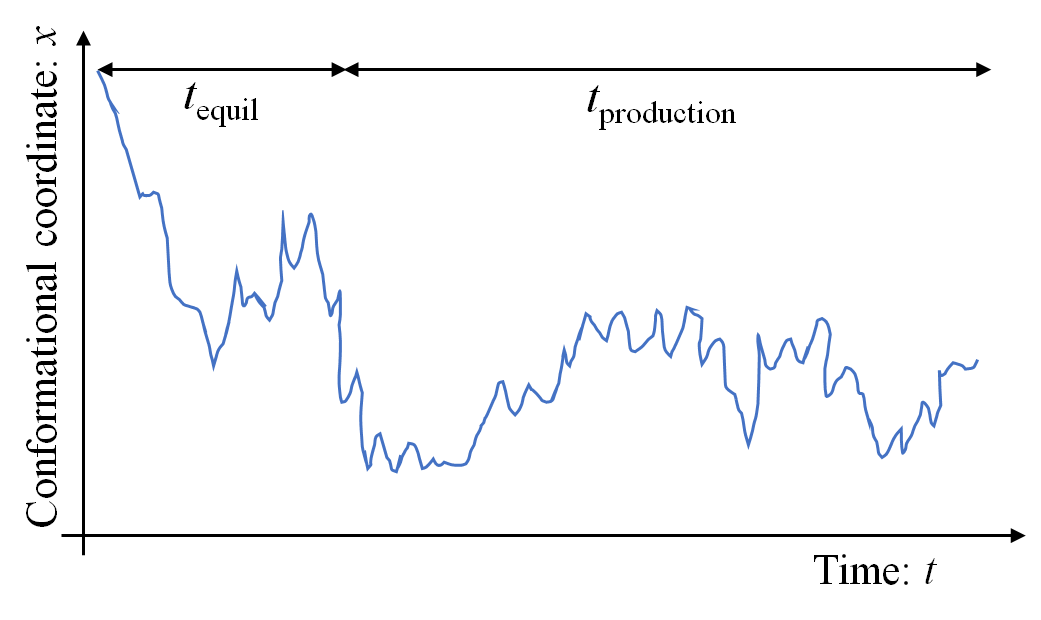
\includegraphics[width=7cm]{figures/tequil-time-trace}
  \caption{
  \label{fig:tequil}
  The equilibration and production segments of a trajectory.
  ``Equilibration'' over the time $t_{\mathrm{equil}}$ represents transient behavior while the initial configuration relaxes toward configurations more representative of the equilibrium ensemble.
  Readers are encouraged to select $t_{\mathrm{equil}}$ in a systematic way based on published literature.
  If you find strong sensitivity of ``production'' data to the choice of $t_{\mathrm{equil}}$, this suggests additional sampling is required.
  }
\end{figure}

The 'equilibration' or 'burn-in' time $t_{\mathrm{equil}}$ represents the initial part of a single continuous trajectory (whether from MD or MC) that is \emph{discarded} for purposes of data analysis of \emph{equilibrium properties};
the remaining trajectory data is often called `production' data.
See Fig.\ \ref{fig:tequil}.
Discarding data may seem counter-productive, but there is no reason to expect that the initial configurations of a trajectory will be important in the ensemble ultimately obtained.
Including early-time data, therefore, can systematically \emph{bias} results.

In the biomolecular realm, consider the initial configuration of a protein, which has been energy-minimized and otherwise relaxed from a crystal structure.
Such an initial structure might seem to be intrinsically valuable, but remember that configurations important in a crystal environment may not be equally pertinent to an aqueous environment due to e.g. crystal packing etc. Also, any energy minimization/relaxation that has been performed likely will be very local and keep the configuration within or nearby the initial energy basin.  Moreover, the force field used to represent interactions will in general not be identical to that used to as part of the crystal structure solution.
See the RMSD trace in Fig.\ \ref{f:rmsd}, and note the very rapid RMSD increase in the first $\sim$200 ns. Part of this increase is simply entropic: the volume of phase space within 1 {\AA} of a protein structure is extremely small, so the process of thermalizing rapidly increases RMSD from the starting structure, \emph{regardless of how favorable or representative that structure is}.  Thus, examining that initial rapid increase is not helpful in determining an equilibration time.  However, in this case, the RMSD continues to increase past 3 {\AA}, which is larger than the amplitude of simple thermal fluctuations (shown by Fig.\ \ref{f:rmsd}B), indicating an initial drift to a new structure, followed by sampling.

In materials science, if a simulation is designed to study thermally induced fluctuations or defects in a (mostly) ordered system,
an initial fully ordered configuration is not likely to be representative of the targeted ensemble, and the early dynamics represent a transient relaxation toward the average, which is not representative of the desired equilibrium ensemble.

Accepting that some data should be discarded, it is not hard to see that we want to avoid discarding too much data, given that many systems of interest are extremely expensive to simulate.
Putting those two competing goals into statistical language, we want to remove bias but also minimize uncertainty (variance).

Before briefly describing a procedure for estimating the optimal equilibration time, it should be emphasized that the very notion of separating a trajectory into equilibration and production segments
only makes sense if the system has indeed reached configurations important in the equilibrium ensemble.
While it is generally impossible to guarantee this has occurred, some easy checks for determining that this has not occurred are described in Sec.\ \ref{sec:quick}.
\emph{It is essential to perform those basic checks before analyzing data with a more sophisticated approach} that may assume a trajectory has a substantial amount of true equilibrium sampling.

The essential ideas of equilibration analysis are discussed carefully in prior work \cite{Yang2004,Chodera-2016}.
The key procedure is to analyze data as a function of the amount of data removed - i.e., as $t_{\mathrm{equil}}$ increases from zero.
As described by Chodera \cite{Chodera-2016}, both the bias and the variance can be monitored, as well as the effective sample size, which is roughly quantified by the total simulation time considered divided by the auto-correlation time.
Chodera indicates that the effective sample size peaks at the optimal $t_{\mathrm{equil}}$, making the latter easy to discern.
We caution that estimating the correlation time may require care, and readers may want to consider the global 'decrorrelation time' \cite{Lyman2007a} described in Sec.\ \ref{sec:global}.
Further, if values of observables estimated from the production phase depend sensitively on the choice of $t_{\mathrm{equil}}$, it is likely that further sampling is required.
